% The third pattern -- the theory of beating, written from the ground up.
% Build: cd paper && tectonic -X compile paper3.tex --outdir build
%
% This is the shell. The prose is in p3-*.tex, one section per file, one
% new idea per section (paper/notes/paper3-plan.md is the design). Every
% quoted number is a macro in numbers.tex, generated by tools/numbers.mjs,
% which refuses to build over a failing experiment gate.
\documentclass[10pt]{article}
\usepackage[margin=1.1in]{geometry}
\usepackage{amsmath}
\usepackage{amssymb}
\usepackage{amsthm}
\usepackage{booktabs}
\usepackage{graphicx}
\usepackage{xcolor}
\usepackage{microtype}
\usepackage{tikz}
\usepackage{pgfplots}
\pgfplotsset{compat=1.18}
\usetikzlibrary{arrows.meta,decorations.pathreplacing,calc}
\usepackage[most]{tcolorbox}
\usepackage[colorlinks=true, linkcolor=cool, citecolor=cool, urlcolor=cool]{hyperref}
\graphicspath{{figures/}}

\definecolor{ink}{HTML}{15181C}
\definecolor{accent}{HTML}{C81E5A}
\definecolor{cool}{HTML}{1B6CA8}
\definecolor{warm}{HTML}{D4761A}
\definecolor{soft}{HTML}{8A94A0}

\theoremstyle{plain}
\newtheorem{theorem}{Theorem}[section]
\newtheorem{proposition}[theorem]{Proposition}
\newtheorem{lemma}[theorem]{Lemma}
\newtheorem{corollary}[theorem]{Corollary}
\theoremstyle{definition}
\newtheorem{definition}[theorem]{Definition}
\newtheorem{remark}[theorem]{Remark}

% A fact the reader may need from outside the paper: which fact, the one
% consequence used, and the question to type into a search box or an AI.
\newtcolorbox{lookup}[1]{enhanced, colback=cool!4, colframe=cool!55,
  title={Lookup: #1}, fonttitle=\bfseries\small, coltitle=white,
  left=5pt, right=5pt, top=4pt, bottom=4pt, boxrule=0.5pt, arc=1.5pt,
  before skip=8pt, after skip=8pt, fontupper=\small}
% Something the reader can do with objects, a phone, or the app.
\newtcolorbox{tryit}[1]{enhanced, colback=warm!6, colframe=warm!65,
  title={Try it: #1}, fonttitle=\bfseries\small, coltitle=white,
  left=5pt, right=5pt, top=4pt, bottom=4pt, boxrule=0.5pt, arc=1.5pt,
  before skip=8pt, after skip=8pt, fontupper=\small}

\newcommand{\R}{\mathbb{R}}
\newcommand{\Z}{\mathbb{Z}}
\newcommand{\tor}{\mathbb{T}}
\newcommand{\E}{\mathbb{E}}
\newcommand{\cnt}{\xi}
\newcommand{\het}{\eta}
\newcommand{\Moire}{\textsc{Moir\'e}}
\newcommand{\figlead}[1]{\textbf{#1}\ }
\newcommand{\todo}[1]{\textcolor{accent}{[#1]}}

% GENERATED by paper/tools/numbers.mjs -- do not edit by hand.
% Every number the prose quotes, in one place, so text and data cannot drift.

% ---- src/types/moire.ts : what the Studio offers
\newcommand{\fieldCount}{six}
\newcommand{\patternCount}{thirteen}
\newcommand{\envTaps}{24}

% ---- data/fringe.json : the fringe law
\newcommand{\fringeScenes}{12}
\newcommand{\fringeSamples}{107{,}691}
\newcommand{\fringeMeanErr}{0.0034}
\newcommand{\fringeWorstP}{0.073}
\newcommand{\fringeLight}{0.036}
\newcommand{\fringeDark}{0.416}
\newcommand{\fringeRegime}{1/4}

% ---- data/lawatlas.json : admitted fraction per panel
\newcommand{\atlasCombs}{100.0}
\newcommand{\atlasCircleLines}{39.1}
\newcommand{\atlasHex}{93.5}
\newcommand{\atlasCircles}{21.7}
\newcommand{\atlasControl}{0.0}

% ---- data/gradient.json : the missing gradient divide
\newcommand{\gradWorstWave}{25.2}
\newcommand{\gradWorstHyp}{14.8}
\newcommand{\gradWorstSpiral}{7.3}
\newcommand{\gradWorstParab}{224}
\newcommand{\gradWaveFrame}{61}
\newcommand{\gradHypFrame}{66}
\newcommand{\gradParabFrame}{98}
\newcommand{\gradSpiralFrame}{0}

% ---- data/gpu.json : 1200x800 = 0.96 Mpixel, one full-screen layer
\newcommand{\gpuSpeedLo}{11}
\newcommand{\gpuSpeedHi}{37}
\newcommand{\gpuTriRotOne}{14.4}
\newcommand{\gpuTriRotOneNew}{0.39}
\newcommand{\gpuTriRotOffOut}{27.9}
\newcommand{\gpuTriRotOffOutNew}{1.64}
\newcommand{\gpuSquareOld}{0.92}
\newcommand{\gpuSquareClosed}{0.20}
\newcommand{\gpuSquareClosedGain}{4.7}
\newcommand{\gpuAdapter}{metal-3}

% ---- data/gpu.json : interpreting a field expression against unrolling it
\newcommand{\interpPerOp}{0.103}
\newcommand{\interpLo}{0.63}
\newcommand{\interpHi}{6.9}
\newcommand{\interpHiOps}{67}
\newcommand{\unrolledLo}{0.0043}
\newcommand{\unrolledCeil}{0.054}
\newcommand{\fieldBaseline}{0.0071}
\newcommand{\fieldEmptyCost}{0.044}
\newcommand{\fieldEmptyGain}{6}
\newcommand{\fieldOpsLo}{6}
\newcommand{\fieldOpsHi}{67}
\newcommand{\fieldStmtHi}{73}
\newcommand{\fieldTwinWorst}{4{\times}10^{-5}}
\newcommand{\fieldGainLo}{40}
\newcommand{\fieldGainHi}{265}

% ---- data/cost.json : CPU metric evaluations per pixel, mean
\newcommand{\costScenes}{7}
\newcommand{\costSweepLo}{180}
\newcommand{\costSweepHi}{361}
\newcommand{\costOursLo}{7.5}
\newcommand{\costOursHi}{11.1}
\newcommand{\costVsSweepLo}{18}
\newcommand{\costVsSweepHi}{33}
\newcommand{\costVsRefLo}{1.7}
\newcommand{\costVsRefHi}{9.4}

% ---- data/artifacts.json
\newcommand{\artHolesSweepDiff}{8.6}
\newcommand{\artHolesSweepEv}{1100}
\newcommand{\artHolesOursEv}{72}
\newcommand{\artHolesSaving}{15}
\newcommand{\artDriftLooseDiff}{38.3}
\newcommand{\artDriftRefInk}{0.459}
\newcommand{\artDriftLooseInk}{0.152}
\newcommand{\artAnchorEv}{33}
\newcommand{\artAnchorRefInk}{0.489}
\newcommand{\artAnchorLatticeInk}{0.216}
\newcommand{\artAnchorPixelInk}{0.216}

% ---- data/fidelity.json : the sweep against the exhaustive reference
\newcommand{\fidSettings}{2{,}401}
\newcommand{\fidLegible}{1{,}534}
\newcommand{\fidSweepHoles}{160}
\newcommand{\fidSweepWorst}{32.9}
\newcommand{\fidSweepLegibleHoles}{3}
\newcommand{\fidSweepLegibleWorst}{4.2}
\newcommand{\fidSweepEnvelopeHoles}{41}
\newcommand{\fidSweepEnvelopeWorst}{29.6}
\newcommand{\fidLooseHoles}{46}
\newcommand{\fidLooseWorst}{48.3}
\newcommand{\fidLooseEnvelopeHoles}{13}
\newcommand{\fidOursHoles}{146}
\newcommand{\fidOursWorst}{13.8}

% ---- data/saturation.json : the interval-width sweep
\newcommand{\satSettings}{55{,}692}
\newcommand{\satFitting}{45{,}774}
\newcommand{\satFittingPct}{82}
\newcommand{\satStrided}{9{,}918}
\newcommand{\satWidestFitting}{1022}
\newcommand{\satMedianInk}{0.89}
\newcommand{\satStridedLegible}{1{,}472}
\newcommand{\satStridedLegiblePct}{2.6}
\newcommand{\satBudget}{1{,}024}
\newcommand{\satDriftRatioHi}{4.2}

% ---- data/degenerate.json : strided band against a deep scan
\newcommand{\degChecked}{534}
\newcommand{\degWithDrop}{217}
\newcommand{\degWorst}{48.8}
\newcommand{\degMean}{4.6}
\newcommand{\degLegible}{298}
\newcommand{\degLegibleWorst}{28.7}

% ---- data/residual.json : the worked pixel of the window figure
\newcommand{\figNaive}{49}
\newcommand{\figTrue}{41}
\newcommand{\figGap}{8}
\newcommand{\figLo}{22}
\newcommand{\figHi}{56}
\newcommand{\figSpan}{35}
\newcommand{\figEvals}{9}
\newcommand{\figGuard}{10.5}
\newcommand{\figSpacing}{14}

% ---- data/window.json : the interval checked against a brute-force argmin
\newcommand{\winChecks}{13{,}458}
\newcommand{\winViolations}{0}

% ---- data/ablation.json : one mechanism removed, time relative to full
\newcommand{\ablSkipLo}{2.1}
\newcommand{\ablSkipHi}{3.3}
\newcommand{\ablClosedMarginal}{90.3}
\newcommand{\ablCostLo}{8}
\newcommand{\ablCostHi}{19}
\newcommand{\ablMpixel}{3.84}

% ---- data/zoom.json : zoom stability
\newcommand{\zoomDecades}{1.2}
\newcommand{\zoomRefSamples}{36}
\newcommand{\zoomCoarsestPeriod}{1.5}
\newcommand{\zoomFloorNoise}{0.046}
\newcommand{\zoomNoFloorNoise}{0.115}
\newcommand{\zoomValueNoise}{0.118}
\newcommand{\zoomFloorNoiseCoarse}{0.002}
\newcommand{\zoomNoFloorNoiseCoarse}{0.115}
\newcommand{\zoomNoiseRatio}{77}
\newcommand{\zoomFloorInkGain}{0.61}
\newcommand{\zoomValueBias}{0.004}

% ---- data/contour.json : moire as a contouring primitive
\newcommand{\contourCarrier}{5}
\newcommand{\contourDetune}{5.5556}
\newcommand{\contourCtlGap}{50}
\newcommand{\contourFloor}{0.22}
\newcommand{\contourFloorP}{0.61}
\newcommand{\contourBestErr}{0.23}
\newcommand{\contourWorstErr}{0.58}
\newcommand{\contourAtFloor}{three}
\newcommand{\contourAtFloorErr}{0.25}
\newcommand{\contourFieldCount}{six}
\newcommand{\contourWorstP}{2.62}
\newcommand{\contourProbes}{63{,}904}
\newcommand{\contourFinest}{8.14}
\newcommand{\contourDipoleResolved}{86}
\newcommand{\contourDipoleFinest}{8.14}


\title{The third pattern\\[0.3em]\large How beats emerge from counting}
\author{}
\date{Draft, \today}

\begin{document}
\maketitle

\begin{abstract}
Lay two rulers of slightly different pitch side by side and a slow pattern
of coincidences appears that is on neither ruler. Feed two trains of clicks
through a detector that fires only when clicks coincide and it fires at the
difference of the rates and at nothing else. Print two gratings over each
other and broad bands appear that survive blurring, photographing and bad
printing. This paper is about that third pattern: what it is, why every
observer that averages before it decides must see it, which of the many
possible patterns wins, and in what precise sense it is a new thing that
the parts do not contain. The tool is elementary. Give every family of
repeated members a \emph{count} --- how many members up to here,
interpolated --- and a superposition becomes a point moving on a torus, a
picture painted on that torus, and nothing else. The pattern you see is the
picture averaged along the fast directions of the torus; that average is a
function of the slow combinations of counts alone, it has a closed form,
and it does not depend on the observer, only on the geometry. From this one
fact follow predictions that were not built in and that we measure: a
stroke of duty one half extinguishes the octave beat of gratings and of
sounds alike; a beat in the air needs a nonlinear ear while a beat on paper
needs none; hard-edged patterns look the same to every observer and blurred
ones do not; beats of beats are heard only by observers with two stages;
and some ratios of pitches, the golden ratio first among them, never beat
visibly at any order. Every number in the paper is generated by a script
that fails if the prediction does. Frequencies are never needed. Counting
is what beating is.
\end{abstract}

\section{Coincidence}
\label{sec:coincidence}

Three things you can do this afternoon.

\paragraph{Two rulers.}
Take a ruler with ten divisions to the inch and lay it edge to edge against
one with nine. Somewhere along the pair a tick of the first sits exactly on a
tick of the second. Move your eye along. The next pair of ticks is a hair
apart, the next a hair more, and after ten ticks of the first ruler and nine
of the second the ticks coincide again. What you see, without trying, is a
slow pattern of near-coincidences that repeats every inch. It is on neither
ruler. Nothing about it needs to be exact, either: bend the rulers a little,
or space the ticks slightly unevenly, and the pattern of coincidences is
still there, slightly uneven in its own way.

\paragraph{Two click trains.}
Now sound. Two trains of clicks at nearly equal rates, say a hundred and a
hundred and one per second, go into a detector that fires only when two
clicks arrive together. Clicks arrive together once per second, so the
detector fires once per second. That is the difference of the two rates,
and it is all the detector knows. Raise both trains to a thousand and a
thousand and one clicks per second and the detector's output is
\emph{exactly} the same, one click per second; it never learned the
original rates at all. The sum of the two trains, as a signal, contains
nothing that repeats once per second. The detector makes it.

\paragraph{Two gratings.}
Print a grating of fine lines on a transparency, print another with a
slightly different spacing, and lay one over the other. From arm's length
you see broad bands, much wider than the lines. Blur your eyes: the bands
stay, and the lines go. Photograph the pair out of focus, threshold the
photograph to pure black and white, print it badly: the bands are always in
the same place. Only their contrast changes.

\paragraph{What the three share.}
Each family comes in numbered members: ticks, clicks, lines. The pattern
that emerges is a pattern of \emph{coincidences} between the numbering of
one family and the numbering of the other. It lives on a scale set by how
slowly the two numberings drift apart, and it is read out by anything that
\emph{pools} --- an eye, a detector, a blur --- with the pooling changing
only how strongly the pattern shows, never where it is. None of the three
descriptions used the word frequency, and the second example does not even
have a stable one. What the three have is a count.

\begin{definition}[The count]
\label{def:count}
A \emph{family} is anything that comes in numbered members along a line, a
plane, a circle or a clock: ticks, clicks, lines, rings, teeth, steps, days.
Its \emph{count} $\cnt(x)$ is the number of members up to the point $x$,
interpolated between members, so that $\cnt$ is a whole number exactly on a
member and $\cnt=n+\tfrac12$ halfway from member $n$ to member $n+1$.
\end{definition}

For a ruler of pitch $T$ the count is $\cnt(x)=x/T$: ten members to the inch
means $\cnt$ rises by ten per inch. But the count exists for any family,
evenly spaced or not, and that is the whole reason this paper never needs a
frequency. A frequency says where a family is on average. A count says where
it is here. Figure~\ref{fig:rulers} draws both rulers with their counts and
the one number that the pattern of coincidences depends on: the difference
of the two counts.

\begin{figure}[t]
  \centering
  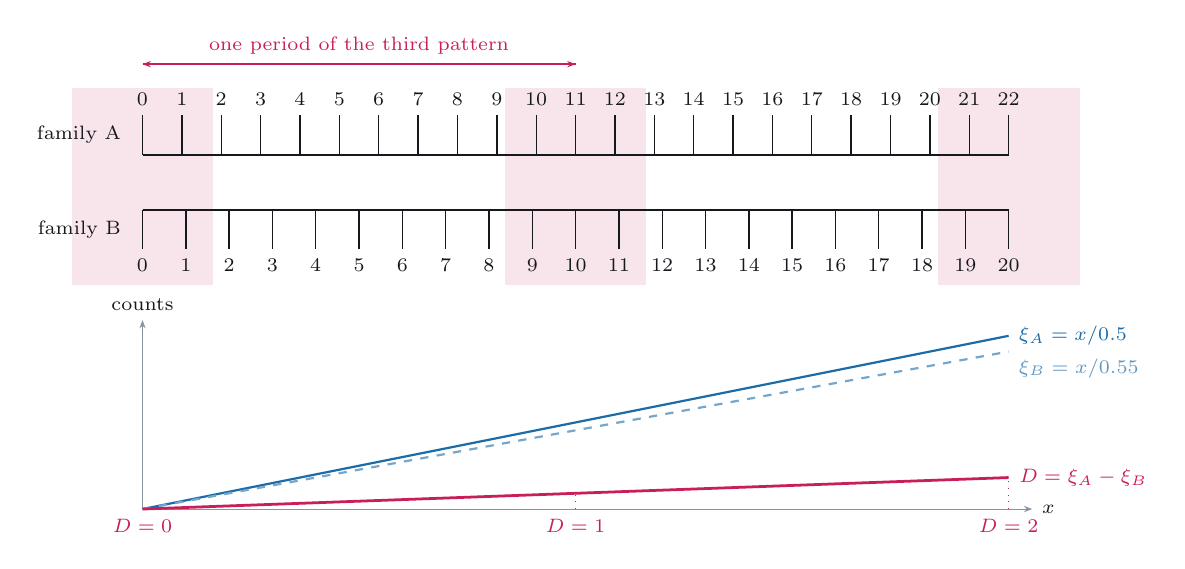
\begin{tikzpicture}[x=1cm, y=1cm, font=\scriptsize, >={Stealth[length=3pt]}]
    % Bands where the ticks nearly coincide: the third pattern.
    \foreach \c in {0, 5.5, 11} {
      \fill[accent!12] ({\c-0.9},-0.05) rectangle ({\c+0.9},2.45);
    }
    % Ruler A: pitch 0.5 (10 per "inch" of 5 units): ticks at 0.5 k.
    \draw[ink, line width=0.6pt] (0,1.6) -- (11,1.6);
    \foreach \k in {0,...,22} {
      \draw[ink, line width=0.5pt] ({0.5*\k},1.6) -- ({0.5*\k},2.1);
      \node[ink, above=0pt] at ({0.5*\k},2.1) {\k};
    }
    \node[ink, anchor=east] at (-0.15,1.85) {family A};
    % Ruler B: pitch 0.55 (9 per 5 units): ticks at 0.55 k.
    \draw[ink, line width=0.6pt] (0,0.9) -- (11,0.9);
    \foreach \k in {0,...,20} {
      \draw[ink, line width=0.5pt] ({0.55*\k},0.9) -- ({0.55*\k},0.4);
      \node[ink, below=0pt] at ({0.55*\k},0.4) {\k};
    }
    \node[ink, anchor=east] at (-0.15,0.65) {family B};
    % One period of the pattern.
    \draw[accent, ->, line width=0.6pt] (0,2.75) -- (5.5,2.75) node[midway, above, accent] {one period of the third pattern};
    \draw[accent, ->, line width=0.6pt] (5.5,2.75) -- (0,2.75);
    % The counts, and their difference, as small plots below.
    \begin{scope}[shift={(0,-2.9)}]
      \draw[soft, ->] (0,0) -- (11.3,0) node[right, ink] {$x$};
      \draw[soft, ->] (0,0) -- (0,2.4) node[above, ink] {counts};
      \draw[cool, line width=0.8pt] (0,0) -- (11,2.2) node[right, cool] {$\cnt_A=x/0.5$};
      \draw[cool!60, line width=0.8pt, dashed] (0,0) -- (11,2.0) node[right, cool!70, yshift=-6pt] {$\cnt_B=x/0.55$};
      \draw[accent, line width=1pt] (0,0) -- (11,0.4) node[right, accent] {$D=\cnt_A-\cnt_B$};
      \foreach \c/\v in {5.5/1, 11/2} {
        \draw[accent, dotted] (\c,0) -- (\c,{0.2*\v});
        \node[accent, below] at (\c,0) {$D=\v$};
      }
      \node[accent, below] at (0,0) {$D=0$};
    \end{scope}
  \end{tikzpicture}
  \caption{\figlead{Two rulers and the one number that matters.} Family A
  has ten members where family B has nine. Above: the rulers, with their
  members numbered; the shaded bands are where a member of A falls near a
  member of B, the pattern that is on neither ruler. Below: the two counts
  $\cnt_A$ and $\cnt_B$ rise at slightly different rates, and their
  difference $D=\cnt_A-\cnt_B$ rises slowly. The bands sit exactly where $D$
  is a whole number. The pattern repeats when $D$ has grown by one, which
  takes ten members of A and nine of B: the drawing is the definition of a
  vernier, and everything in this paper is a generalisation of it.}
  \label{fig:rulers}
\end{figure}

\paragraph{What this paper claims.}
Every superposition of families is a point moving on a torus, plus a fixed
picture painted on the torus (\S\ref{sec:torus}). Any observer that pools
before it decides --- a blur, an exposure, an ear, a detector --- sees the
picture averaged along the torus's fast directions, and that average is a
function of the \emph{slow combinations of counts} alone; it has a closed
form, and the observer's own nonlinearity changes the picture but never the
geometry (\S\ref{sec:pooling}). Which of the possible combinations shows is
a question of arithmetic with a classical answer and a twist
(\S\ref{sec:selection}). The pattern that emerges has its own count, so it
can beat again, and the hierarchy is exact (\S\ref{sec:iterated}). Counts
can fail to exist in exactly three ways, and each way has a signature
(\S\ref{sec:counting}). Everything with a number attached is measured
(\S\ref{sec:ledger}), most of it in a drawing tool built for the purpose
(\S\ref{sec:instrument}), and the predictions that reach outside drawings
--- into sound, into strobes, into anything that counts --- are the point.

\begin{tryit}{the rulers}
Two rulers with different units work (centimetres against sixteenths of an
inch is a good pair), or two combs, or two pieces of window screen laid
over each other and turned slowly. Count how many members of each family fit
in one period of the bands. In Figure~\ref{fig:rulers} that is ten and nine;
the rule you will find is that the two counts differ by exactly one per
period, whatever the families are.
\end{tryit}

\section{Where you are in every family}
\label{sec:torus}

Stand at a point $x$ on the pair of rulers. You are, say, three tenths of the
way from tick 40 to tick 41 of family A, and seven tenths of the way from
tick 36 to tick 37 of family B. Those two fractions, $0.3$ and $0.7$, are
where you are \emph{within the current member} of each family, and they are
all a pattern of coincidences can depend on: whether ticks coincide at $x$ is
a question about the fractions, not about the numbers 40 and 36.

\begin{definition}[The torus of counts]
\label{def:torus}
For $K$ families with counts $\cnt_1,\dots,\cnt_K$ the \emph{state} of the
superposition at $x$ is the point
\[
  \Phi(x)=\big(\cnt_1(x),\dots,\cnt_K(x)\big)\bmod 1,
\]
the fractional part of every count at once. For two families $\Phi(x)$ is a
point $(u_1,u_2)$ of the unit square. Walking off the right edge of the
square (family A completes a member) brings you back in at the left edge at
the same height, and walking off the top brings you back in at the bottom:
the square with its opposite edges glued is a \emph{torus}, written
$\tor^2$, and as $x$ moves, $\Phi(x)$ traces a path on it.
\end{definition}

\begin{lookup}{the torus as a square with its edges glued}
What to look up: \emph{why a square with opposite edges identified is called
a torus}. The one consequence this paper uses: a function on the torus is
the same thing as a function $I(u_1,u_2)$ of two ordinary variables that
repeats with period one in each variable separately. Nothing about the
torus's shape in three dimensions is ever used; only the gluing.
\end{lookup}

The state says where things are. What they look like is a separate thing,
and separating the two is the first idea worth having.

\begin{definition}[The picture on the torus]
\label{def:picture}
What the superposition \emph{looks like} at $x$ --- how much ink, how loud,
whether the detector fires --- depends on $x$ only through the state
$\Phi(x)$, by a fixed rule $I$ that knows nothing about $x$: the
\emph{picture on the torus}. The superposition is the composite
\[
  S \;=\; I\circ\Phi,\qquad S(x)=I\big(\Phi(x)\big).
\]
\end{definition}

The formula says: look up where you are in every family, then look up what
that state looks like. For two printed gratings $I(u_1,u_2)$ is ``ink if
$u_1$ is within the stroke of a line of A, or $u_2$ within a line of B'' ---
a picture on the torus made of two bands, one across and one up, and their
crossing. For two click trains into a coincidence detector $I(u_1,u_2)$ is
``fire if $u_1$ and $u_2$ are both within a click's width of zero'', a small
square at the corner of the torus. Everything about \emph{where} ---
pitches, spacings, the bend in a ruler, a drift in a clock --- lives in
$\Phi$. Everything about \emph{what} --- ink, click shape, brightness,
whether inks multiply or sounds add --- lives in $I$. Two superpositions
with the same $\Phi$ differ only in their picture, and two with the same
picture differ only in their state map. The rest of the paper is a list of
things that are properties of $\Phi$, things that are properties of $I$, and
things that are properties of the way an observer averages one over the
other.

\begin{figure}[t]
  \centering
  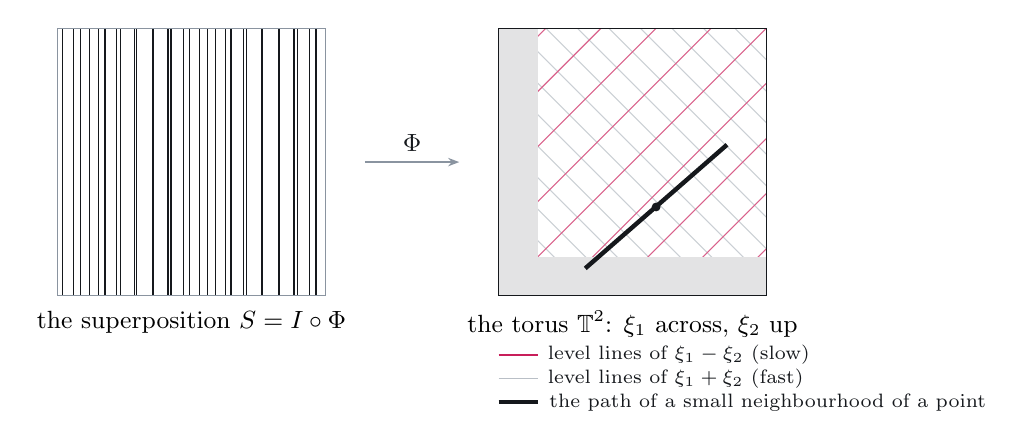
\begin{tikzpicture}[x=1cm, y=1cm, font=\small, >={Stealth[length=4pt]}]
    \begin{scope}
      \clip (0,0) rectangle (3.4,3.4);
      \foreach \i in {0,...,17} { \draw[ink, line width=0.45pt] ({\i*0.2},0) -- ({\i*0.2},3.4); }
      \foreach \i in {0,...,15} { \draw[ink, line width=0.45pt] ({\i*0.23+0.06},0) -- ({\i*0.23+0.06},3.4); }
    \end{scope}
    \draw[soft] (0,0) rectangle (3.4,3.4);
    \node[below=2pt] at (1.7,0) {the superposition $S=I\circ\Phi$};
    \draw[->, soft, thick] (3.9,1.7) -- (5.1,1.7) node[midway, above, ink] {$\Phi$};
    \begin{scope}[shift={(5.6,0)}]
      \clip (0,0) rectangle (3.4,3.4);
      \foreach \c in {0.4,0.8,...,6.8} { \draw[soft!45, thin] (\c,0) -- (0,\c); }
      \foreach \c in {-2.8,-2.1,...,2.8} { \draw[accent!70, thin] (\c,0) -- (\c+3.4,3.4); }
      \fill[ink!12] (0,0) rectangle (0.5,3.4);
      \fill[ink!12] (0,0) rectangle (3.4,0.5);
      % A neighbourhood's path: along the fast direction, whose slope is the
      % ratio of the two families' rates, 0.2/0.23 = 0.87.
      \draw[ink, line width=1.6pt] (1.1,0.35) -- (2.9,1.92);
      \fill[ink] (2.0,1.13) circle (1.6pt);
    \end{scope}
    \draw[ink] (5.6,0) rectangle (9,3.4);
    \node[below=2pt] at (7.3,0) {the torus $\tor^2$: $\cnt_1$ across, $\cnt_2$ up};
    \draw[accent, thin] (5.6,-0.75) -- (6.1,-0.75) node[right, ink, font=\scriptsize] {level lines of $\cnt_1-\cnt_2$ (slow)};
    \draw[soft!60, thin] (5.6,-1.05) -- (6.1,-1.05) node[right, ink, font=\scriptsize] {level lines of $\cnt_1+\cnt_2$ (fast)};
    \draw[ink, line width=1.6pt] (5.6,-1.35) -- (6.1,-1.35) node[right, ink, font=\scriptsize] {the path of a small neighbourhood of a point};
  \end{tikzpicture}
  \caption{\figlead{A superposition beside its torus.} Left: two families of
  lines a little apart in pitch. Right: the torus of their counts. The
  picture $I$ is the two shaded bands, a line of A across and a line of B
  up; ink at a point of the plane is $I$ looked up at that point's state.
  A small neighbourhood of a point maps to a short segment on the torus
  (black), pointing in the direction in which both counts advance --- the
  \emph{fast direction}. The level lines (contour lines) of $\cnt_1-\cnt_2$
  run nearly along the segment, so that combination barely changes across a
  neighbourhood; the level lines of $\cnt_1+\cnt_2$ are crossed many
  times. The first is slow and the second fast, and the whole theory is about
  what is slow.}
  \label{fig:torus}
\end{figure}

\subsection{Combined counts, and which of them are slow}
\label{sec:slow}

The difference $D=\cnt_A-\cnt_B$ of Figure~\ref{fig:rulers} is itself a
count: it rises by one per period of the bands, and the bands are its
members. So is the sum $\cnt_A+\cnt_B$, and so is any combination
\[
  k\cdot\cnt \;=\; k_1\cnt_1+k_2\cnt_2+\dots+k_K\cnt_K,
  \qquad k=(k_1,\dots,k_K)\ \text{whole numbers},
\]
a whole number of one count plus a whole number of another. The formula says:
combined counts are made of the counts by integer recipes, and the recipe is
the vector $k$. We write $k=(1,-1)$ for the difference, $(1,1)$ for the sum,
$(2,-1)$ for twice the first count minus the second. A combined count is a
count in its own right --- it runs upward like $D$ in Figure~\ref{fig:rulers}
--- and its fractional part depends only on the state $\Phi(x)$, because a
whole-number combination of whole numbers is a whole number. Every recipe is
a candidate pattern, all of them at once. Which ones show is a matter of how
fast each changes.

Here is why recipes with entries bigger than one matter, in one sentence
that \S\ref{sec:whosees} unpacks. A family with sharp edges, seen as a
function of its own count, is a sum of waves that repeat once, twice, three
times per member --- its \emph{harmonics} --- and the second harmonic of
family A against the first of family B makes a pattern of coincidences with
recipe $(2,-1)$, as surely as the first against the first makes $(1,-1)$.
A pair of rulers with ten and nineteen divisions to the inch shows it:
twice the first count minus the second rises by one per inch, and that is
the pattern you see, faint but there. Nineteen to ten is nearly two to one,
the ratio of an octave in music, so we call $(2,-1)$ the \emph{octave}
recipe.

\begin{definition}[Slow and fast; the heterodyne ratio]
\label{def:eta}
At a point $x$ each count has a local rate, its derivative $\nabla\cnt_i(x)$
--- a number on a line, a vector in the plane, giving members per unit of
distance. The rate of a combined count is $\nabla(k\cdot\cnt)=\sum_ik_i\nabla\cnt_i$.
For a recipe $k=(a,b)$ on two families, its \emph{heterodyne ratio} is
\[
  \het_{a,b}(x)\;=\;\frac{\lvert a\,\nabla\cnt_1+b\,\nabla\cnt_2\rvert}
                        {\tfrac12\big(\lvert a\,\nabla\cnt_1\rvert+\lvert b\,\nabla\cnt_2\rvert\big)},
\]
the rate of the combination divided by the average rate of the two
harmonics that form it. Its reciprocal is the number of members per band.
A recipe is \emph{slow} when $\het$ is small; we call $\het<\tfrac14$, more
than four members per band, the \emph{beat regime}, and it is where every
pattern in this paper lives.
\end{definition}

The word is the radio engineer's: to \emph{heterodyne} is to mix two rates
and keep their difference, and $\het$ says how clean the mix is. On the
rulers of Figure~\ref{fig:rulers}, with rates $10$ and $9$ per inch, the
difference has $\het=1/9.5$, nine and a half members per band, and the sum
has $\het=19/9.5=2$: half a member per band, which is no band at all. The
click trains of \S\ref{sec:coincidence} have rates $100$ and $101$ per
second and $\het=1/100.5$ for the difference; a hundred clicks per pulse.
Turn one ruler around so that its count runs the other way, and the sum
becomes the slow one; nothing in the theory prefers a difference. The
threshold $\tfrac14$ is where a pattern of coincidences stops being one:
with more than four members per band the bands are wider than the members
that make them, and with fewer there is no ``band'', only members. The
ratio is a number at every point of the plane, so it can be drawn as a map,
and the tool of \S\ref{sec:instrument} draws it: bright where no pattern can
form, dark where one must. From here on the members themselves --- the
ticks, the clicks, the lines, the fine texture a pooling observer loses ---
are the \emph{carrier}, radio's word again, and a slow recipe is a
\emph{beat}.

\begin{table}[t]
  \centering\small
  \begin{tabular}{@{}lll@{}}
    \toprule
    Symbol & Read it as & Introduced \\
    \midrule
    $\cnt_i(x)$ & the count of family $i$ up to $x$ & Definition~\ref{def:count} \\
    $\Phi(x)$ & the state: where you are in every family, on the torus $\tor^K$ & Definition~\ref{def:torus} \\
    $u=(u_1,u_2)$ & a point of the torus; $x$ is always a point of the line or plane & Definition~\ref{def:torus} \\
    $I$ & the picture on the torus: what a state looks like & Definition~\ref{def:picture} \\
    $S=I\circ\Phi$ & the superposition itself & Definition~\ref{def:picture} \\
    $k=(k_1,\dots,k_K)$ & a recipe: whole numbers & \S\ref{sec:slow} \\
    $k\cdot\cnt$ & the combined count with recipe $k$ & \S\ref{sec:slow} \\
    $D$ & the difference of two counts, recipe $(1,-1)$ & Figure~\ref{fig:rulers} \\
    $\het$ & the heterodyne ratio: one over the members per band & Definition~\ref{def:eta} \\
    $\hat I(k)$ & the strength of recipe $k$'s wave in the picture & \S\ref{sec:sweep} \\
    $w$, $\mathcal E_w$ & a slide (a recipe of whole numbers) and the average along it & Theorem~\ref{thm:sweep} \\
    $\E[\,I\mid\text{slow}\,]$ & the picture averaged over everything the slow recipes do not fix & \S\ref{sec:sweep} \\
    $T_I(D)$ & the tent: the average as a function of $D$ & Corollary~\ref{cor:cases} \\
    $W$, $\rho$, $\widehat W$ & an observer's window, its width, and its response to a wave & \S\ref{sec:window} \\
    $N$ & an observer's front end: what it does to each value before pooling & \S\ref{sec:observer} \\
    $O$ & an observer: a front end, then a window, then anything & Theorem~\ref{thm:universality} \\
    \bottomrule
  \end{tabular}
  \caption{\figlead{Every symbol in the paper}, and where it is introduced.
  The lower half is used from \S\ref{sec:pooling} on.}
  \label{tab:symbols}
\end{table}

\begin{tryit}{the map of where a beat can form}
In \Moire\ (\S\ref{sec:instrument}), make two layers of parallel lines a few
percent apart in pitch and turn on the \emph{ratio} view. The frame darkens
where $\het<\tfrac14$: the bands you see in the ordinary view sit exactly
inside the dark region, and as you change the pitches the dark region
predicts where the bands go before they get there. Rotate one layer: the
dark region moves to where the \emph{sum} is slow, and the bands follow.
\end{tryit}

\section{What pooling sees}
\label{sec:pooling}

Blur your eyes at the two gratings and the lines go while the bands stay.
Point a camera at two gratings sliding past each other and leave the shutter
open: the lines smear away and the bands are what the film records. Listen
to the two click trains through a detector too slow to follow the clicks:
what comes out is the once-per-second pulse. In every case an observer that
\emph{pools} --- averages over a stretch of space or time before it responds
--- keeps the pattern of coincidences and loses the members. This section
says exactly what such an observer sees, and the answer is short: the
picture on the torus, averaged along the fast directions.

\subsection{The sharp version: one period of every family}
\label{sec:sweep}

Why talk about sliding when the observer blurs? Because on the torus the two
are the same motion. Blurring averages the superposition over a small
neighbourhood of $x$; across that neighbourhood every count advances a
little, all of them together, so the neighbourhood's states form a short
segment on the torus in the fast direction, the black segment of
Figure~\ref{fig:torus}, and averaging over the neighbourhood is averaging
the picture along that segment. A blur is a short slide with soft ends.
The cleanest pooling observer is therefore one that averages over
\emph{exactly one member of every family}. Slide both gratings by one line
each, at the same rate, and average the ink you saw along the way. On the
torus that slide is the straight path from $\Phi(x)$ in the direction
$(1,1)$ back to $\Phi(x)$: one unit across, one unit up, and the gluing
brings it home. The average of the picture along that closed path is what
the observer sees at $x$.

\begin{theorem}[One period of every family is a sharp average]
\label{thm:sweep}
Let $w=(w_1,\dots,w_K)$ be a recipe of whole numbers, and slide family $i$
through $w_i$ of its members while averaging:
\[
  \mathcal E_w I(\Phi)\;=\;\int_0^1 I\big(\Phi+u\,w\big)\,du .
\]
Then $\mathcal E_w I$ depends on the state $\Phi$ only through the combined
counts whose recipe is orthogonal to the slide,
$k\cdot w=k_1w_1+\dots+k_Kw_K=0$. In words: sliding every family through a
whole number of members keeps exactly the recipes that the slide does not
change, and removes every other, completely.
\end{theorem}

The idea of the proof: write the picture as a sum of waves on the torus, one
per recipe; the slide carries each wave round a whole number of times, and
a wave carried round a whole number of times averages to nothing unless it
was not carried round at all. The lookup makes both halves of that sentence
concrete.

\begin{lookup}{waves on the torus}
What to look up, in this order. First, \emph{Euler's formula}: the number
$e^{2\pi i\theta}$ is the point of the unit circle at angle $\theta$ turns,
so as $\theta$ runs from $0$ to $1$ the point goes once round the circle,
and its average position over a whole number of turns is the centre, $0$
--- while for zero turns it stays at $1$. That is the one integral the
reader has to believe: for a whole number $m$, $\int_0^1e^{2\pi imu}\,du$ is
$1$ if $m=0$ and $0$ otherwise. Second, \emph{Fourier series}: a function
that repeats with period one in each of its variables is a sum of such
waves, one per whole-number recipe,
$I(u)=\sum_k\hat I(k)\,e^{2\pi i\,k\cdot u}$, with coefficients $\hat I(k)$
that say how much of each wave the picture contains. A recipe's wave on
the torus, pulled back to the plane, is a wave in the combined count
$k\cdot\cnt$. Nothing else from Fourier analysis is used anywhere in the
paper.
\end{lookup}

\begin{proof}
Expand $I(\Phi+uw)=\sum_k\hat I(k)\,e^{2\pi i\,k\cdot\Phi}\,e^{2\pi i\,u\,(k\cdot w)}$.
Because $k$ and $w$ are whole-number vectors, $m=k\cdot w$ is a whole number,
and the integral over $u$ of $e^{2\pi i m u}$ is $1$ for $m=0$ and $0$
otherwise. What survives is $\sum_{k\cdot w=0}\hat I(k)\,e^{2\pi i\,k\cdot\Phi}$,
which is a function of the recipes with $k\cdot w=0$ and of nothing else.
\end{proof}

The theorem is a statement about an average, and the right name for the
average is a \emph{conditional expectation}: $\mathcal E_wI$ is the average of
the picture over everything the kept recipes do not fix. We write it
$\E[\,I\mid\text{slow}\,]$, ``the picture, given the slow recipes'', and the
word means nothing more than that here; the slow recipes are the ones the
slide keeps, $k\cdot w=0$. What is remarkable is the word \emph{exactly}
in the statement. The slide is by a whole number of members, so every wave
it does not keep is carried round a whole number of times and cancels to
zero, with nothing left over. A slide by a fraction of a member would leave
a little of everything.

\begin{corollary}[Four things the theorem already says]
\label{cor:cases}
\begin{enumerate}
\item \emph{The tent.} Two families slid together, $w=(1,1)$: the kept
recipes are $(a,-a)$, so the average is a function of the difference $D$
alone, $\mathcal E_wI=T_I(D)$, where $T_I(\Delta)=\int_0^1 I(v,v-\Delta)\,dv$
is the picture averaged along the diagonal line that sits $\Delta$ below the
main one. For two strokes it is the saturating tent of Figure~\ref{fig:tent}:
flat where one stroke lies inside the other, rising at unit slope while
they separate, flat again once they clear. Not a sine.
\item \emph{The mean.} (A remark rather than a case, since the theorem
wants whole numbers.) A slide whose rates have no common measure, averaged
for a long time, keeps only $k=0$: the plain mean of the picture, the ink
with every family's phase independent of every other's.
\item \emph{Every zero-sum at once.} The diagonal slide $w=(1,\dots,1)$ keeps
every recipe whose entries sum to zero: every difference of two counts and
every three-family recipe like $(1,1,-2)$, all at the same time. A recipe
whose entries do not sum to zero, like the octave $(2,-1)$, needs a slide of
its own, $w=(1,2)$.
\item \emph{A long exposure is a slide.} Animate the families at whole-number
rates $r=(r_1,\dots,r_K)$ members per second and expose for one second: the
film records $\mathcal E_rI$. The shutter keeps exactly the recipes with
$k\cdot r=0$, and which pattern the photograph shows is a matter of
arithmetic.
\end{enumerate}
\end{corollary}

\begin{figure}[t]
  \centering
  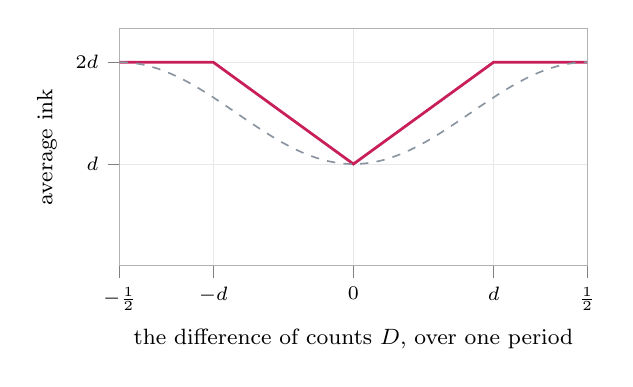
\begin{tikzpicture}
    \begin{axis}[width=0.62\linewidth, height=4.6cm,
      xlabel={the difference of counts $D$, over one period}, ylabel={average ink},
      xmin=-0.5, xmax=0.5, ymin=0, ymax=0.7,
      xtick={-0.5,-0.3,0,0.3,0.5}, xticklabels={$-\tfrac12$,$-d$,$0$,$d$,$\tfrac12$},
      ytick={0.3,0.6}, yticklabels={$d$,$2d$},
      tick align=outside, tick pos=left, axis line style={gray!60},
      grid=major, grid style={gray!18, very thin},
      label style={font=\footnotesize}, tick label style={font=\scriptsize}, samples=201]
      \addplot[accent, line width=1pt, domain=-0.5:0.5] {0.6 - max(0, 0.3 - abs(x))};
      \addplot[soft, dashed, line width=0.6pt, domain=-0.5:0.5] {0.45 - 0.15*cos(deg(2*pi*x))};
    \end{axis}
  \end{tikzpicture}
  \caption{\figlead{What pooling sees for two strokes: a tent, not a sine.}
  Two families of strokes, each covering a fraction $d$ of its pitch, slid
  through one member each and averaged, as a function of the difference of
  counts $D$. Where $D$ is a whole number the strokes lie on each other and
  the ink is $d$; as they separate the ink rises at unit slope; once they
  clear, at $|D|=d$, it saturates at $2d$ and stays there. The dashed curve is
  the sine that a theory of sinusoids would predict. The flat top is why a
  beat of strokes looks crisp. Note the sign: Figure~\ref{fig:rulers} shaded
  the coincidences, and on paper a coincidence is where the strokes
  overlap and the ink is \emph{least}, so the light bands of a printed pair
  are the coincidences. The depth of the tent is $d$ until the strokes
  cover half their pitch and shrinks after, which is why thickening a pen
  past half the pitch only darkens the page.}
  \label{fig:tent}
\end{figure}

Case 4 is a physical prediction, and it was not sought: it fell out of the
theorem and was measured the same afternoon. The measurement is in
Figure~\ref{fig:exposure}. Two families of lines at pitches $16.4$ and $8$
carry an octave beat, recipe $(2,-1)$, a few percent of the ink and
invisible on a still under the lines themselves. Animate them at rates
$(1,2)$ --- the slide that keeps $(2,-1)$ --- and expose for one period: the
octave beat is kept to \exposureFaithfulPct\% of its strength on the still.
Animate at $(1,1)$ or $(2,1)$ and the same exposure washes it away,
$\exposureSelectivity\times$ down. The photograph is not post-processing. It is
what a slow observer of a moving pair already computes.

\begin{figure}[t]
  \centering
  
\includegraphics[width=\linewidth]{exposure-quad.png}
  \caption{\figlead{The shutter is a filter on recipes.} The $16.4{:}8$ pair
  as a still, then its long exposures over one period at rates $(1,1)$,
  $(1,2)$ and $(2,1)$; in each exposure the departures from its own average
  ink are multiplied by six so that a few-percent pattern shows on the page.
  Rates $(1,1)$ keep the zero-sum recipes --- here the carrier-scale
  $(1,-1)$, a fine texture, not a band --- and wash the octave; rates $(1,2)$
  keep exactly the octave $(2,-1)$, the broad bands; rates $(2,1)$ wash both
  and keep the faster $(1,-2)$. Scripts \texttt{exposure.mjs},
  \texttt{exposure-figs.mjs}.}
  \label{fig:exposure}
\end{figure}

\subsection{The soft version: a window}
\label{sec:window}

An eye does not slide anything by exactly one member. It blurs: it averages
the superposition over a small neighbourhood, with some weight $W$ that is
large at the centre and falls off at a distance $\rho$. What does a blur see?
The same thing, softly. Along the neighbourhood's segment on the torus each
combined count advances at its own rate, and a blur of width $\rho$ kills a
wave whose rate is fast compared with $1/\rho$ and keeps a wave whose rate
is slow: it applies to each recipe the blur's own response at that recipe's
local rate.

\begin{lookup}{what a blur does to a wave}
What to look up: \emph{the Fourier transform of a window} (or: ``what does
convolving with a Gaussian do to $\cos(2\pi\nu x)$''). Blurring $S$ with a
window $W$ means replacing $S(x)$ by the weighted average of $S$ near $x$,
written $S*W$ (a \emph{convolution}). The consequence used: averaging a
wave of rate $\nu$ with a symmetric window $W$ of width $\rho$ multiplies
the wave by a number $\widehat W(\rho\nu)$ --- the window's \emph{response}
--- which is $1$ at $\nu=0$ and falls to nearly $0$ once $\rho\nu$ is more
than about one; in the plane the rate is a vector and the response is that
of the window to a plane wave with that rate vector. The window's
\emph{second moment} $m_2$ is the average of $|y|^2$ under it, a measure of
its width. A low-pass filter is the same statement in time.
\end{lookup}

\begin{theorem}[A window is a multiplier on the torus]
\label{thm:multiplier}
Let $W$ be a symmetric window of total weight one and second moment $m_2$,
and $W_\rho$ the same window stretched to width $\rho$. Write $\nu_k(x)$ for
the local rate of the combined count $k\cdot\cnt$ at $x$, and $\kappa$ for
the largest second derivative of the counts (how curved the state map is).
If the picture's waves are summable, $\sum_k|k|\,|\hat I(k)|<\infty$, then
\[
  (S*W_\rho)(x)\;=\;\sum_k \hat I(k)\;\widehat W\!\big(\rho\,\nu_k(x)\big)\;
  e^{2\pi i\,k\cdot\Phi(x)}\;+\;R(x),
  \qquad
  |R(x)|\;\le\;\pi\,\kappa\,m_2\,\rho^2\sum_k|k|\,|\hat I(k)| .
\]
In words: a blur sees the picture on the torus with each recipe's wave
multiplied by the window's response \emph{at that recipe's own local rate},
plus a remainder that is second order in the width of the blur and
proportional to the curvature of the state map.
\end{theorem}

The idea of the proof: near $x$ the state map is nearly straight, so across
the neighbourhood each recipe's wave is nearly a plain wave at its local
rate, and a window answers a plain wave with its response; the only error
is the curvature of $\Phi$, which is what the remainder measures.

\begin{proof}
Expand $I$ in waves and write $\Phi(y)=\Phi(x)+J(y-x)+E(y)$, where $J$ is
the matrix whose rows are the rates $\nabla\cnt_i(x)$ and $E$ is the
curvature term, $|E(y)|\le\tfrac12\kappa|y-x|^2$. The window average of
$e^{2\pi i\,k\cdot J(y-x)}$ is the response $\widehat W(\rho\,\nu_k(x))$,
because $k\cdot J(y-x)=\nu_k(x)\cdot(y-x)$ is the combined count's rate
times the displacement. The factor $e^{2\pi i\,k\cdot E(y)}$ differs from
$1$ by at most $2\pi|k|\,|E(y)|$, which averages against $W_\rho$ to at most
$\pi|k|\,\kappa\,m_2\rho^2$; summing over $k$ gives the bound on $R$.
\end{proof}

When the local rates split cleanly --- the fast ones well above $1/\rho$,
the slow ones well below, which is the beat regime $\het\ll1$ --- the
multiplier is nearly $1$ on the slow recipes and nearly $0$ on the fast, and
the blur reports $\E[\,I\mid\text{slow}\,](\Phi(x))$: the same conditional
expectation as the sharp slide, with the window's small leakage in place of
the slide's exact zero. The identity is measured to $\obsMultiplierErr$ on a
geometry without curvature, and with curvature the remainder is accounted
for by the multiplier's own second derivative to within
$\obsRemainderResidual$ of itself (script \texttt{observer.mjs}). The
textbook explanation of the bands of two printed gratings as ``what
survives a blur'' is this theorem's soft case, said once per point rather
than once per picture.

\subsection{The observer theorem}
\label{sec:observer}

An eye is not a blur. A photoreceptor saturates, an ear rectifies, a
detector thresholds, a film has a gamma: real observers apply some
\emph{front end} $N$ to the signal at each instant, and pool afterwards. The
coincidence detector of \S\ref{sec:coincidence} is the extreme case, a front
end that outputs nothing unless both clicks are present. Does a front end
change where the pattern is?

\begin{lemma}[A front end changes the picture, never the geometry]
\label{lem:transport}
For any function $N$ of one number, $N\circ(I\circ\Phi)=(N\circ I)\circ\Phi$.
\end{lemma}

This is just the associativity of composition, and it is the most useful
line in the paper. Applying $N$ to the superposition is the same as applying
$N$ to the picture on the torus and then looking that new picture up at the
same state. The state map $\Phi$, and with it every combined count and every
rate and every value of $\het$, is untouched. Which recipes are slow, and
where, is a property of the geometry that no observer can change. An
observer chooses only its picture.

\begin{theorem}[Universality of the third pattern]
\label{thm:universality}
Let an observer $O$ be any front end $N$ followed by any pooling window
$W_\rho$, followed by anything at all. Then at every point $x$ it reports the
picture $N\circ I$ filtered by the multiplier of
Theorem~\ref{thm:multiplier}, and in the beat regime
\[
  O(S)(x)\;=\;\E\big[\,N\circ I\;\big|\;\text{slow}\,\big]\big(\Phi(x)\big).
\]
The set of slow recipes is the geometry's alone. An observer chooses only
the picture it averages and the leakage of its window.
\end{theorem}

\begin{proof}
Lemma~\ref{lem:transport} turns the observer into a blur of the
superposition with picture $N\circ I$, whose coefficients satisfy the
summability condition whenever $N$ is smooth and $I$'s do;
Theorem~\ref{thm:multiplier} applies. Whatever is applied after the window
acts on a function of the result and cannot reintroduce a recipe the
window removed.
\end{proof}

Order matters, and the theorem says how. An observer that pools first and
responds after, applying some $g$ to the blurred value, sees
$g(\E[I\mid\text{slow}])$: the plain average with its contrast re-mapped, a
function of the slow counts and so carrying no recipe outside the kept
set. An observer that responds first, $W_\rho\circ N$, sees the average of
a \emph{different picture} $N\circ I$: the same slow recipes, with different
strengths, and possibly recipes the original picture never carried at all
--- \S\ref{sec:whosees} shows a picture with no beat in it acquiring one
this way. Both are averages of a picture on the same torus along the same
fast directions. That is the precise sense in which the third pattern is
not the observer's: every observer that pools before it decides reports an
average along the fast directions, and only the picture is its own. The
next section is about what an observer's picture can and cannot contain,
and it is where the theory leaves the page and enters the ear.

\begin{tryit}{a long exposure}
Two combs, or two pieces of window screen, one held still and one moved
steadily across it, photographed with a phone in night mode or any
long-exposure setting. The members smear to grey; the bands survive, and
move at the rate the count difference changes: if the moving screen
advances one member per second, the bands advance one band per second.
Move the second screen at twice the speed of the first, both moving, and a
different set of bands survives: Corollary~\ref{cor:cases}, case 4, on a
kitchen table.
\end{tryit}

\section{Who can see a beat}
\label{sec:whosees}

Return to the click trains. Two trains of clicks in the air \emph{add}: the
pressure at your eardrum is the sum of the two. Two gratings printed on
transparencies and held to the light \emph{multiply}: light gets through
where both are clear, and the transmission is the product. Two gratings
thrown on a wall by two projectors add again. The difference sounds like
bookkeeping and is the whole reason a beat in the air needs an ear and a
beat on paper does not.

On the torus the two cases are two pictures. If family 1 has profile $g_1$
(one where a click or a stroke is, zero between) and family 2 has $g_2$,
then an additive superposition has the picture $I(x_1,x_2)=g_1(x_1)+g_2(x_2)$
and a multiplicative one has $I(x_1,x_2)=g_1(x_1)\,g_2(x_2)$. Everything
follows from expanding each in waves.

\begin{lookup}{the waves of a pulse train}
What to look up: \emph{the Fourier coefficients of a rectangular pulse
train} (or ``Fourier series of a square wave with duty cycle $d$''). The
consequences used: a train that is on for a fraction $d$ of each period has
coefficients $\hat g(n)=\sin(n\pi d)/(n\pi)$ for $n\ne0$ and $\hat g(0)=d$;
so $\hat g(n)$ is exactly zero when $nd$ is a whole number (a $50\%$ train
has no even harmonics at all), and otherwise $|\hat g(n)|$ falls like
$1/n$.
\end{lookup}

\begin{theorem}[Who sees a beat]
\label{thm:whosees}
Write a recipe $k=(a,b)$ as \emph{cross} when both $a$ and $b$ are nonzero.
\begin{enumerate}
\item An additive picture $g_1(x_1)+g_2(x_2)$ has \emph{no cross recipes}:
its waves are $(n,0)$ and $(0,n)$ only. A linear pooling observer, one that
averages the superposition and nothing more, sees no beat in an additive
superposition, ever.
\item A multiplicative picture $g_1(x_1)\,g_2(x_2)$ carries every cross
recipe with strength $\hat I(a,b)=\hat g_1(a)\,\hat g_2(b)$: a linear
observer sees the beat, with the strength of the two harmonics that make it.
\item A front end that bends, $N''\ne0$, mints cross recipes out of an
additive picture. Squaring the sum gives
$(g_1+g_2)^2=g_1^2+2g_1g_2+g_2^2$, whose middle term is a product: the
difference recipe $(1,-1)$ appears with strength $\hat g_1(1)\hat g_2(1)/2$
when the sum is normalised to $(g_1+g_2)/2$.
\end{enumerate}
\end{theorem}

\begin{proof}
A wave on the torus with recipe $(a,b)$ is $e^{2\pi i(ax_1+bx_2)}$. The
expansion of $g_1(x_1)$ contains only waves $e^{2\pi i\,n x_1}$, recipes
$(n,0)$, and likewise $g_2$; a sum of the two contains nothing else, which
is the first claim, and by Theorem~\ref{thm:sweep} any average that removes
the single-family recipes removes everything. The product of two expansions
is the sum over all pairs of the products of waves, and
$e^{2\pi i\,ax_1}e^{2\pi i\,bx_2}$ is the wave of recipe $(a,b)$ with
coefficient $\hat g_1(a)\hat g_2(b)$, which is the second. Expanding the
square gives the third, the cross term $2g_1g_2$ contributing
$2\hat g_1(a)\hat g_2(b)$ at $(a,b)$, and the normalisation divides by four.
\end{proof}

Measured: the additive beat under a linear observer is $\obsAdditiveBeat$,
zero to the precision of the arithmetic; the printed beat is
$\obsPrintedBeat$; a squaring front end mints the additive beat at
$\obsSquaringBeat$, exactly half the printed value; a saturating front end
$\min(g_1+g_2,1)$, the front end of a photoreceptor or a clipping amplifier,
mints it at $\obsSaturatingBeat$, nearly the printed value
(script \texttt{observer.mjs}).

This is the coincidence detector of \S\ref{sec:coincidence}, explained. A
detector that fires only when both clicks are present is a front end that
multiplies --- ``both'' is a product --- so its picture on the torus is the
small square where both counts are near a whole number, a picture with
every cross recipe in it, and the slowest cross recipe is the difference of
counts $D$. The detector's output is a wave in $D$, once per unit of $D$,
once per second, and nothing else survives its pooling. It is also
Helmholtz's combination tone~\cite{Helmholtz1954Sensations}: two tones in
the air have no difference tone between them until an ear, which is not
linear before it pools, makes one. The distinction is not between kinds of
observer. It is between kinds of superposition, and the theorem puts it in
the only place it can be: which recipes the observer's picture contains.

\subsection{Hard patterns are observer-proof, soft ones are not}
\label{sec:hardsoft}

\begin{corollary}[Hard patterns]
\label{cor:hard}
If the picture $I$ takes only two values, then for any front end $N$,
\[
  N\circ I \;=\; N(0)+\big(N(1)-N(0)\big)\,I ,
\]
a constant plus a multiple of $I$: every observer sees the same recipes at
the same relative strengths, and differs from every other only by a
constant and a gain. A hard-edged pattern --- ink or no ink, click or no
click --- has one third pattern, and every observer sees it.
\end{corollary}

The proof is the display: a function of a variable that takes two values is
determined by its two values, and any such function is affine. Measured: the
octave null of \S\ref{sec:selection} under a linear and a squaring observer
agree to $\obsHardNull$.

\begin{corollary}[Soft patterns]
\label{cor:soft}
Blur the edges of a $50\%$ train symmetrically, by any even smoothing. Its
even harmonics stay exactly zero, so every \emph{linear} observer keeps the
null at every blur. A squaring observer does not: it reopens the null with
a strength that grows linearly in the width of the blur.
\end{corollary}

\begin{proof}
A $50\%$ train satisfies $g(x+\tfrac12)=1-g(x)$; a symmetric smoothing
preserves this half-turn antisymmetry, and a function with it has no even
harmonics. Squaring destroys the antisymmetry exactly on the blurred edges
and nowhere else, so the even harmonics it mints scale with the edge width.
\end{proof}

Measured on strokes with anti-alias ramps of half-width \obsReopenRamps\
units: the linear null holds at every ramp, and squaring reopens it at
$\obsReopenAmps$, linear in the ramp (\texttt{observer.mjs}).

\subsection{The same theorem in an ear}
\label{sec:ear}

Everything so far was measured in a drawing tool. The theorem does not know
that. Take two pulse trains at $200$ and $405$ clicks per second --- a
mistuned octave, whose slow recipe is $(2,-1)$, twice the lower count minus
the upper, beating five times a second --- add them as sounds add, and
listen through four model ears: a low-pass filter alone (a linear ear),
a squaring front end followed by the low-pass (the textbook square-law
detector), a cubing front end, and a two-stage ear that squares, pools,
and squares again. Sweep the lower train's duty from $30\%$ to $70\%$ and
read the five-hertz line at the output. Figure~\ref{fig:ear} is the result
(script \texttt{ear.mjs}).

\begin{figure}[t]
  \centering
  \begin{tikzpicture}
    \begin{axis}[width=0.5\linewidth, height=5.4cm, ymode=log,
      title={hard pulses}, xlabel={duty of the lower train},
      ylabel={the 5 Hz line at the ear's output},
      xmin=0.27, xmax=0.73, ymin=1e-7, ymax=1,
      xtick={0.3,0.4,0.5,0.6,0.7},
      tick align=outside, tick pos=left, axis line style={gray!60},
      grid=major, grid style={gray!18, very thin},
      label style={font=\footnotesize}, tick label style={font=\scriptsize},
      title style={font=\footnotesize},
      legend style={font=\scriptsize, draw=gray!40, at={(0.5,-0.32)}, anchor=north, legend columns=2}]
      \addplot[soft, mark=x, line width=0.6pt] table[x=duty, y=hard_linear, col sep=comma]{data/ear-octave.csv};
      \addlegendentry{linear}
      \addplot[accent, mark=*, mark size=1.2pt, line width=0.7pt] table[x=duty, y=hard_squarelaw, col sep=comma]{data/ear-octave.csv};
      \addlegendentry{square-law}
      \addplot[cool, mark=square*, mark size=1.1pt, line width=0.7pt] table[x=duty, y=hard_cubic, col sep=comma]{data/ear-octave.csv};
      \addlegendentry{cubic}
      \addplot[warm, mark=triangle*, mark size=1.3pt, line width=0.7pt] table[x=duty, y=hard_squarepoolsquare, col sep=comma]{data/ear-octave.csv};
      \addlegendentry{square, pool, square}
    \end{axis}
  \end{tikzpicture}%
  \hfill%
  \begin{tikzpicture}
    \begin{axis}[width=0.5\linewidth, height=5.4cm, ymode=log,
      title={softened pulses}, xlabel={duty of the lower train},
      xmin=0.27, xmax=0.73, ymin=1e-7, ymax=1,
      xtick={0.3,0.4,0.5,0.6,0.7}, yticklabels={},
      tick align=outside, tick pos=left, axis line style={gray!60},
      grid=major, grid style={gray!18, very thin},
      label style={font=\footnotesize}, tick label style={font=\scriptsize},
      title style={font=\footnotesize}]
      \addplot[accent, mark=*, mark size=1.2pt, line width=0.7pt] table[x=duty, y=soft_squarelaw, col sep=comma]{data/ear-octave.csv};
      \addplot[cool, mark=square*, mark size=1.1pt, line width=0.7pt] table[x=duty, y=soft_cubic, col sep=comma]{data/ear-octave.csv};
      \addplot[warm, mark=triangle*, mark size=1.3pt, line width=0.7pt] table[x=duty, y=soft_squarepoolsquare, col sep=comma]{data/ear-octave.csv};
    \end{axis}
  \end{tikzpicture}
  \caption{\figlead{The octave beat through four ears.} Two pulse trains at
  $200$ and $405$ per second, added as sounds add, through a linear ear, a
  square-law ear, a cubic ear and a two-stage ear, as the lower train's duty
  is swept. Left, hard-edged pulses: the linear ear hears nothing at any
  duty (Theorem~\ref{thm:whosees}, first claim), and every nonlinear ear
  hears the beat except at duty one half, where it is extinguished
  $\earHardNullSquare\times$, $\earHardNullCubic\times$ and
  $\earHardNullCascade\times$ under the three ears --- a hard pattern is
  observer-proof (Corollary~\ref{cor:hard}). Right, the same pulses with
  softened edges: the square-law ear keeps the null ($\earSoftNullSquare\times$),
  the cubic ear reopens it to within $\earSoftNullCubic\times$ of its
  neighbours (Corollary~\ref{cor:soft}, where cubing plays the part of
  squaring one order up). Script \texttt{ear.mjs}, data \texttt{ear.json}.}
  \label{fig:ear}
\end{figure}

Three things in the figure were predictions before they were curves. The
linear ear hears no beat at any duty, $\earLinearOverSquare$ of what the
square-law ear hears, because a sum of trains has no cross recipe. Every
nonlinear ear loses the beat at duty one half, because the beat rides the
lower train's second harmonic and a $50\%$ train has none: the same duty
null that \S\ref{sec:selection} measures on paper, in sound, through three
different ears at once. And softening the pulses separates the ears: a
square-law front end's cross term is a product of one harmonic from each
train, so it inherits the lower train's missing second harmonic and keeps
the null; a cubic front end's $g_1^2g_2$ term carries the \emph{square} of
the lower train, whose second harmonic is not zero once the edges are soft,
and the null reopens. That is a prediction about people: \emph{which
nonlinearity an ear has is audible}, in a mistuned octave of blurred square
waves, as the presence or absence of a five-hertz beat. We have not done the
listening test. \S\ref{sec:ledger} says exactly what it would take.

\begin{tryit}{a beat that a duty can switch off}
Any synthesizer with a pulse-width control, or a free web synth. Two
oscillators, pulse waves, at $200$ and $405$ hertz; set the lower one's
width to $30\%$ and you hear a five-per-second throb; set it to $50\%$ and
the throb goes, though both tones are still there; $70\%$ and it is back.
Your ear is the nonlinearity. Then put a gentle low-pass filter on each
oscillator, so the edges soften, and listen at $50\%$ again: if you hear the
throb come back, your ear's front end is not a square-law.
\end{tryit}

\section{Which pattern emerges}
\label{sec:selection}

Every recipe is present in a multiplicative picture, and a bent front end
puts most of them into an additive one. Which of them do you see? Two
ingredients decide it. One is slowness: how small the recipe's heterodyne
ratio is. The other is strength: how much of the picture the recipe
carries, which for anything with edges falls off with the harmonics. The
theory of two sinusoids --- the textbook theory of beats --- has only the
first ingredient, because a sinusoid has one harmonic and nothing to
choose between; families with edges have both, and the visible pattern is
the one that is slow \emph{per unit of strength}.

\begin{definition}[The priced merit]
\label{def:merit}
For a recipe $(a,b)$ with $ab\ne0$ on two families with local rates
$\nabla\cnt_1$ and $\nabla\cnt_2$, the \emph{priced merit} is the heterodyne
ratio of Definition~\ref{def:eta} charged the product of the harmonic
orders that carry the recipe,
\[
  \mu_{a,b}\;=\;\het_{a,b}\cdot|ab|
  \;=\;\frac{\lvert a\,\nabla\cnt_1+b\,\nabla\cnt_2\rvert}
            {\tfrac12\big(\lvert a\,\nabla\cnt_1\rvert+\lvert b\,\nabla\cnt_2\rvert\big)}\cdot|ab| .
\]
The visible recipe is the one with the smallest priced merit, and it shows
as a beat when $\mu<\tfrac14$. For a first-order recipe $\mu=\het$, and the
rule is the four members per band of \S\ref{sec:slow}; a recipe of order
$ab$ is carried by harmonics $ab$ times weaker, and must be $ab$ times
slower to show as strongly.
\end{definition}

The price is Theorem~\ref{thm:whosees}'s second claim read backwards: the
recipe $(a,b)$ is carried by the $a$-th harmonic of one family and the
$b$-th of the other, each about $1/n$ strong, so the beat it makes has
about $1/|ab|$ of the contrast of the first-order beat. Without the price
the question has no answer. Every real ratio of pitches has rational
approximations as good as you like, so at any point some recipe of
enormous order is slower than every other, carried by harmonics no stroke
has --- a pair at the ratio $\sqrt2$ has a recipe $(41,-29)$ with more than
three thousand members per band and nothing to draw them with; with the
price, comparable slowness resolves toward the lower order, and the minimum
is a definite recipe at every point.

\begin{proposition}[Selection is best approximation]
\label{prop:selection}
For two parallel families of pitches $s_1$ and $s_2$, the recipes that beat
every lower-order recipe as the order is allowed to grow are exactly the
convergents of the continued fraction of $s_1/s_2$ (\selRecordsMatch\ of
\selRatios\ ratios measured, without exception). In the plane, where the
rates are vectors, the minimiser is found at every point by
Lagrange--Gauss reduction of the lattice $\{a\nabla\cnt_1+b\nabla\cnt_2\}$
--- the two-dimensional Euclidean algorithm, which finds a lattice's
shortest vectors in a handful of steps~\cite{NguyenStehle2009Gauss} ---
and the reduction names the brute-force winner in $99.8\%$ of
\selTrials\ random pairs (script \texttt{convergents.mjs}).
\end{proposition}

\begin{lookup}{continued fractions}
What to look up: \emph{continued fractions and convergents}, one page of
any number theory text. The facts used: a real $x$ has an expansion
$x=[a_0;a_1,a_2,\dots]$ into whole numbers, its \emph{partial quotients};
truncating gives the fractions $h_n/k_n$, the \emph{convergents} (here
$k_n$ is a denominator, not a recipe), which are the best rational
approximations of $x$ with denominators up to $k_n$; and the error of a
convergent is $|h_n-k_nx|=1/(x_{n+1}k_n+k_{n-1})$, where
$x_{n+1}=[a_{n+1};a_{n+2},\dots]$ is the \emph{complete quotient},
everything after the $n$-th term. For the golden ratio every partial
quotient is $1$; for $\sqrt2$, and for the silver ratio $1+\sqrt2$, every
one after the first is $2$; for $\pi$ they are $3;7,15,1,292,\dots$
\end{lookup}

The proposition is Lagrange's theorem on best approximation with a
different price: the classical statement prices a fraction $h/k$ by $k$,
the priced merit charges $hk$, and the records turn out to be the same
fractions. The reader who takes the one-dimensional case on trust loses
nothing that follows.

\subsection{Duty nulls}
\label{sec:dutynull}

Because a multiplicative picture's strength at a recipe is a product of
harmonics, a station is carried by exactly the harmonics its integers name,
and a family that lacks a harmonic cannot take part in a station that needs
it. That is a prediction the theory of sinusoids cannot make.

\begin{theorem}[Duty nulls]
\label{thm:dutynull}
Let the coarse family's pitch be $a/b$ times the fine family's, in lowest
terms. The visible station is the recipe $(a,-b)$: $a$ coarse counts minus
$b$ fine counts, carried by the coarse family's $a$-th harmonic and the fine
family's $b$-th. A family whose members cover a fraction $d$ of their pitch
has no $a$-th harmonic exactly when $ad$ is a whole number, so the station
is extinguished at those duties of the coarse family and at no others. A
$2{:}1$ pair (coarse pitch twice the fine) has $a=2$, $b=1$: its station
$(2,-1)$ dies at coarse duty $\tfrac12$; a $3{:}1$ pair's station $(3,-1)$
dies at $\tfrac13$ and $\tfrac23$.
\end{theorem}

\begin{proof}
With pitches $s_{\mathrm c}\approx(a/b)\,s_{\mathrm f}$ the combined count
$a\cnt_{\mathrm c}-b\cnt_{\mathrm f}$ has rate
$a/s_{\mathrm c}-b/s_{\mathrm f}\approx b/s_{\mathrm f}-b/s_{\mathrm f}=0$:
it is the slow one, and no recipe of lower order is. By
Theorem~\ref{thm:whosees} its strength is
$\hat g_{\mathrm c}(a)\,\hat g_{\mathrm f}(-b)$, and by the lookup of
\S\ref{sec:whosees}, $\hat g(n)=\sin(n\pi d)/n\pi$ vanishes exactly when
$nd$ is a whole number. A symmetric softening of the edges multiplies each
harmonic by a real factor and moves no zero.
\end{proof}

\begin{figure}[t]
  \centering
  \begin{tikzpicture}
      \begin{axis}[width=0.62\linewidth, height=4.9cm, xlabel={coarse duty $d$},
        ylabel={station strength}, xmin=0.18, xmax=0.82, ymin=0, ymax=0.045,
        scaled y ticks=false, ytick={0,0.01,0.02,0.03,0.04},
        tick align=outside, tick pos=left, axis line style={gray!60},
        grid=major, grid style={gray!18, very thin},
        label style={font=\footnotesize}, tick label style={font=\scriptsize},
        legend style={font=\scriptsize, draw=gray!40, at={(0.5,1.02)}, anchor=south, legend columns=2},
        xtick={0.25,0.333,0.5,0.667,0.75}, xticklabels={$\frac14$,$\frac13$,$\frac12$,$\frac23$,$\frac34$}]
        \addplot[accent, line width=0.7pt] table[x=duty, y=two, col sep=comma]{data/dutynull-law.csv};
        \addlegendentry{$2{:}1$, recipe $(2,-1)$}
        \addplot[cool, line width=0.7pt] table[x=duty, y=three, col sep=comma]{data/dutynull-law.csv};
        \addlegendentry{$3{:}1$, recipe $(3,-1)$}
        \addplot[accent, only marks, mark=*, mark size=1.3pt] table[x=duty, y=two, col sep=comma]{data/dutynull-curve.csv};
        \addplot[cool, only marks, mark=square*, mark size=1.1pt] table[x=duty, y=three, col sep=comma]{data/dutynull-curve.csv};
      \end{axis}
    \end{tikzpicture}\\[4pt]
  
\includegraphics[width=\linewidth]{dutynull-triple.png}
  \caption{\figlead{Duty nulls.} Above: the strength of the station against
  the coarse family's duty, measured on drawn strokes (marks) over the law
  $|\sin(a\pi d)/a\pi|\,|\hat g_{\text{fine}}(1)|$ (lines): the $2{:}1$
  station dies at $d=\tfrac12$, the $3{:}1$ station at $\tfrac13$ and
  $\tfrac23$, and the softened edge of a drawn stroke is the only departure.
  Below: what pooling sees of the $2{:}1$ pair at coarse duty $0.35$, $0.5$
  and $0.65$, expanded sixfold about its mean: present, extinguished,
  present. The nulls are $\dutyNullDepthTwo\times$,
  $\dutyNullDepthThreeLow\times$ and $\dutyNullDepthThreeHigh\times$ deep.
  Scripts \texttt{dutynull.mjs}, \texttt{dutynull-figs.mjs}.}
  \label{fig:dutynull}
\end{figure}

Figure~\ref{fig:dutynull} is the theorem measured on paper;
Figure~\ref{fig:ear} was the same theorem measured in an ear, and
Corollary~\ref{cor:hard}(b) is why the two agree: a hard-edged family has
one set of harmonics, and every observer inherits it. A strobe is a third
place to measure it. A camera taking $f$ frames per second is a family
whose picture is a comb, every harmonic equal, and a wheel whose spokes
pass at $r$ per second beats against it: near $r=f$ the wheel is seen
turning at $r-f$, backwards below the frame rate, the wagon-wheel effect
of every western; at $r=f/2$ consecutive frames sit half a spoke apart, a
pooling eye averages them, and what stands still is a wheel with
\emph{twice} the spokes, carried by the spoke profile's second harmonic.
So a wheel whose spokes are half the gap wide cannot show it. Simulated
on sampled frames (script \texttt{wagonwheel.mjs}): the reversal is exact
to $\wagonReversalErr$, the doubled wheel at spoke duty $0.3$ has contrast
$\wagonDoubledAtThirty$ and tracks $|\sin(2\pi d)/2\pi|$ within
$\wagonLawPct\%$, and at duty $\tfrac12$ it is $\wagonDoubledDepth\times$
down; the tripled wheel at $r=f/3$ dies at duties $\tfrac13$ and
$\tfrac23$ ($\wagonTripledDepthLow\times$, $\wagonTripledDepthHigh\times$).
The frames are simulated and the eye is not; the prediction for a person
is that a wheel with fat spokes never shows the doubled still wheel.

Two readings. Forwards, a band as an instrument: find the duty at which a
station dies and you have measured the family's duty to the precision of
the null. Backwards, a warning about what ``the beat'' is: a $16.4{:}8$
pair also carries the recipe $(1,-2)$, one coarse count minus two fine, a
real coefficient with a period of five units and no band anyone can see,
and the first version of this experiment measured a null of \emph{that}
and called it the station. The station is the slow recipe, not the small
one.

\subsection{Which convergents are stations, and which ratios never beat}
\label{sec:stations}

\begin{proposition}[Stations are the convergents with large complete quotients]
\label{prop:stations}
Let a pair have pitch ratio $x=[a_0;a_1,a_2,\dots]$ with convergents
$h_n/k_n$ and complete quotients $x_{n+1}$. The priced merit of the recipe
$(h_n,-k_n)$ is exactly
\[
  \mu_n\;=\;\frac{2\,h_nk_n}{(h_n+k_nx)\,(x_{n+1}k_n+k_{n-1})},
\]
and the convergent is a station, $\mu_n<\tfrac14$, exactly when
$x_{n+1}+k_{n-1}/k_n>8/(1+k_nx/h_n)$, a bound within a few percent of $4$.
A next partial quotient $a_{n+1}\ge5$ guarantees a station and
$a_{n+1}\le2$ forbids one. For the golden ratio $\mu_n\to1/\sqrt5$, for
$\sqrt2$ and the silver ratio it tends to $1/2\sqrt2$: none of those pairs
has a station at any order.
\end{proposition}

\begin{proof}
Put the convergent's error $|h_n-k_nx|=1/(x_{n+1}k_n+k_{n-1})$ from the
lookup into the merit $2hk\,|h-kx|/(h+kx)$; that is the identity. The
threshold rearranges $\mu_n<\tfrac14$. Since $a_{n+1}<x_{n+1}<a_{n+1}+1$
and $0\le k_{n-1}/k_n<1$, a partial quotient of five or more puts the left
side above $5$ and the right side is at most $8$ over $1$-and-a-bit; a
partial quotient of two or less keeps the left side below $4$, and the
small amount by which the right side can fall short of $4$, which is the
convergent's own error, is smaller still for every denominator beyond the
first few, a case check the script does. For the golden ratio every
complete quotient is the golden ratio $\varphi$ itself and
$k_{n-1}/k_n\to1/\varphi$, so $\mu_n\to1/(\varphi+1/\varphi)=1/\sqrt5$; for
$\sqrt2$ the complete quotients are $1+\sqrt2$ and $k_{n-1}/k_n\to\sqrt2-1$.
\end{proof}

The identity is, up to a factor that tends to one, a classical quantity
(Perron's $k_n|k_nx-h_n|$), and $1/\sqrt5$ is Hurwitz's
constant~\cite{Hurwitz1891Annaherung, Khinchin1964Continued}: the theory of
which beats are visible turns out to be the theory of how well a number can
be approximated, priced slightly differently. What is new is the threshold,
which reads a pair's stations off its partial quotients, and the
\emph{deserts}: a ratio whose partial quotients stay small never beats
visibly at any order, however rich the families' harmonics. Measured on
\stationsConvergents\ convergents of \stationsRatios\ random ratios, the
identity agrees with the tool's own scan to $\stationsIdentityErr$, the
limit holds to $\stationsPerronErr$ past the sixth convergent, the
partial-quotient rules hold without exception, the golden ratio's merit
tends to \stationsGoldenMerit\ and the silver ratio's to
\stationsSilverMerit, both above $\tfrac14$ (\texttt{stations.mjs}).
Table~\ref{tab:stations} reads the proposition on five pairs. The desert is
in sound too: two sawtooth tones --- every harmonic present, falling like
$1/n$ --- at $200$ and $410$ hertz, the ratio $2.05$, carry a station line
at ten hertz through a square-law ear that is $\earDesertRatio\times$
stronger than the strongest slow line of two sawtooths at $200$ hertz and
$200$ times the golden ratio (\texttt{ear.mjs}). The prediction for
hearing: golden intervals of harmonic-rich tones sound rough, but they
never \emph{beat}.

\begin{table}[t]
  \centering\small
  % GENERATED by paper/tools/numbers.mjs -- do not edit by hand.
\begin{tabular}{@{}llp{0.52\linewidth}@{}}
\toprule
Pair & Ratio & First convergents; stations in bold \\
\midrule
$16.4{:}8 = 41{:}20$ & 2.0500 & \textbf{2/1}, \textbf{41/20} \\
$15{:}5$, one turned $2^\circ$ & 2.9982 & 2/1, \textbf{3/1}, \textbf{1640/547}, 8203/2736, 26249/8755, \dots \\
$\sqrt2$ & 1.4142 & 1/1, 3/2, 7/5, 17/12, 41/29, \dots \\
$e$ & 2.7183 & 2/1, 3/1, 8/3, 11/4, \textbf{19/7}, \dots \\
$\pi$ & 3.1416 & \textbf{3/1}, \textbf{22/7}, 333/106, \textbf{355/113}, 103993/33102, \dots \\
\bottomrule
\end{tabular}

  \caption{\figlead{Stations, read off the continued fraction.} For each
  pair, the first convergents of its pitch ratio; the ones the threshold
  makes visible stations are in bold. $\pi$ beats at $3$, $22/7$ and
  $355/113$, because its partial quotients $7$, $15$ and $292$ are large;
  $e$ at $19/7$ and later at $193/71$; $\sqrt2$, whose quotients are all
  $2$, at nothing; the $41{:}20$ pair at its octave. Generated from
  \texttt{stations.json}.}
  \label{tab:stations}
\end{table}

\begin{figure}[t]
  \centering
  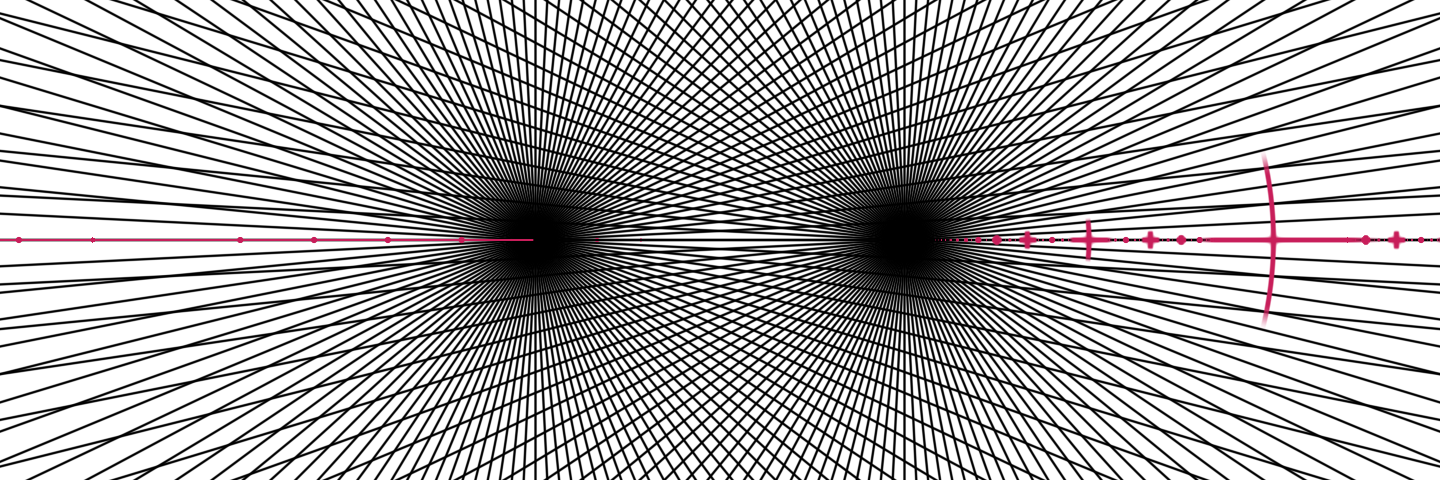
\includegraphics[width=\linewidth]{selection-stations.png}
  \caption{\figlead{Stations as places.} Two fans of rays from two centres.
  Along the axis between them the local ratio of the two families' rates
  sweeps through the reals, every rational the price admits owns a stretch
  of the axis where its recipe is the slow one, and the marks show where
  each station's bands are: the ladder of convergents laid out as
  geography. A pair whose ratio varies has its stations at places, not at
  settings. Script \texttt{selectionfigs.mjs}.}
  \label{fig:stations}
\end{figure}

\begin{tryit}{a station you can switch off with a marker}
Two rulers, or two drawn combs, at pitches close to $2{:}1$ --- ten and
nineteen to the inch --- show octave bands. Now thicken the coarse comb's
ticks with a marker until each covers half the gap: the bands vanish while
both combs are plainly still there. Thicken them to two thirds and the
bands come back. In \Moire, two layers of lines at pitches $16.4$ and $8$
with the coarse stroke at width $8.2$ do the same thing in the pooled view,
and the \emph{ratio} view shows the station's region going blank.
\end{tryit}

\section{Emergence, iterated}
\label{sec:iterated}

The bands of Figure~\ref{fig:rulers} are a family. They have members, the
bands; they have a count, which is the difference $D$ itself, rising by one
per band; and they have a profile, the tent of Figure~\ref{fig:tent}. So
they can beat. Lay a third ruler beside the first two, at a pitch such that
its count runs close to $D$, and a pattern of coincidences forms between
the third family and the \emph{bands}: a beat of a beat. This section says
when that happens, who can see it, and in what precise sense the pattern
that emerges is a new thing.

\begin{proposition}[Averages compose]
\label{prop:tower}
For two slides $w$ and $w'$, averaging along $w$ and then along $w'$ is the
same as averaging over both at once: it keeps exactly the recipes with
$k\cdot w=0$ and $k\cdot w'=0$. Pooling observers stacked in a cascade keep
smaller and smaller sets of recipes, and the set at each stage is the
intersection of the sets before it.
\end{proposition}

\begin{proof}
By Theorem~\ref{thm:sweep} the first average multiplies the wave of
recipe $k$ by $1$ if $k\cdot w=0$ and $0$ otherwise, and the second does the
same with $w'$; the product of the two indicators is the indicator of both
conditions at once.
\end{proof}

So a hierarchy of poolings is a hierarchy of recipe sets, and what a late
stage sees is a pattern in the counts the earlier stages left alone. For
three families the diagonal slide $(1,1,1)$ keeps every recipe whose
entries sum to zero: the three pairwise differences $(1,-1,0)$, $(0,1,-1)$,
$(1,0,-1)$ and, among others, $(1,-2,1)$, the difference of two differences.
That last recipe is the beat of beats, and whether an observer can see it
depends on what its front end can reach.

\begin{theorem}[Beats of beats need a front end of order four]
\label{thm:cascade}
Let three \emph{pure} tones --- sinusoids, each carrying only its first
harmonic --- add, with pairwise slow differences at rates $\delta_1$ and
$\delta_2$ nearly equal. The recipe $(1,-2,1)$, at rate $|\delta_1-\delta_2|$,
has order $|1|+|{-2}|+|1|=4$. A front end that is a polynomial of degree
$n$ mints from pure tones only recipes of order at most $n$, so a
square-law front end ($n=2$) and a cubic one ($n=3$) leave the beat of
beats silent. A cascade that squares, pools, and squares again reaches it,
because its first stage mints the two pairwise beats and its second
multiplies them; so does a single stage of degree four, and a hard
saturation, which is of every degree at once, reaches it weakly. A
multiplicative superposition of the three carries the recipe at linear
order, and a plain blur sees it.
\end{theorem}

\begin{proof}
A pure tone's wave has recipe $\pm1$ in its own count and $0$ in the
others (a real cosine is $\tfrac12(e^{2\pi i\theta}+e^{-2\pi i\theta})$, so
both signs are present). The $n$-th power of a sum of three such waves
expands into monomials $g_1^{e_1}g_2^{e_2}g_3^{e_3}$ with
$e_1+e_2+e_3=n$, and the recipes of such a monomial have $|k_i|\le e_i$,
hence order at most $n$; the recipe $(1,-2,1)$ needs $e_2\ge2$ and
$e_1,e_3\ge1$, four factors, which a square or a cube does not have. The
cascade's first square mints the pairwise differences $(1,-1,0)$ and
$(0,1,-1)$ at order two; the pooling keeps them and removes the rest; the
second square multiplies two real waves, and a product of two real waves
carries both the sum and the difference of their recipes --- the
difference here is $(1,-1,0)-(0,1,-1)=(1,-2,1)$, the beat of beats. A
product of three pictures carries every recipe by
Theorem~\ref{thm:whosees}.
\end{proof}

Measured, on three sinusoids at $300$, $330$ and $363$ hertz --- pairwise
beats at $30$ and $33$, beat of beats at $3$ --- as a fraction of a
first-order beat's strength: a square-law ear hears the three-hertz line
at $\earTernarySquare$, a cubic ear at $\earTernaryCubic$, the cascade at
$\earTernaryCascadePct\%$, and a multiplicative trio through a plain
low-pass at $\earTernaryPrintedPct\%$ (\texttt{ear.mjs};
Figure~\ref{fig:ternary}). The prediction for hearing is that second-order
beats of pure tones are heard only by a system whose front end reaches
order four --- two stages of detection (a front end followed by pooling),
or one stage of high order --- and the psychoacoustics of ``second-order
beats'' has data the theorem constrains; \S\ref{sec:ledger} names it as
the test.

\begin{figure}[t]
  \centering
  \begin{tikzpicture}
    \begin{axis}[width=0.7\linewidth, height=4.6cm, ybar, ymode=log,
      ymin=1e-8, ymax=3, bar width=16pt,
      ylabel={3 Hz line, as a fraction of a first-order beat},
      xtick={0,1,2,3}, xticklabels={square-law, cubic, {square, pool, square}, {multiplied, linear}},
      x tick label style={font=\scriptsize, align=center, text width=2.3cm},
      tick align=outside, tick pos=left, axis line style={gray!60},
      ymajorgrids, grid style={gray!18, very thin},
      label style={font=\footnotesize}, tick label style={font=\scriptsize},
      nodes near coords, point meta=rawy,
      every node near coord/.append style={font=\tiny, /pgf/number format/sci, /pgf/number format/sci generic={mantissa sep=\times,exponent={10^{#1}}}}]
      \addplot[fill=accent!70, draw=accent] table[x=index, y=fraction, col sep=comma]{data/ear-ternary.csv};
    \end{axis}
  \end{tikzpicture}
  \caption{\figlead{The beat of beats, and who hears it.} Three pure tones
  added in the air, listened to through a square-law ear, a cubic ear, and
  a two-stage ear that squares, pools and squares again; and the same three
  families multiplied, through a plain low-pass. The recipe $(1,-2,1)$ has
  order four: one stage of degree two or three cannot mint it from pure
  tones, two stages of degree two can, and a multiplicative superposition
  carries it from the start. Script \texttt{ear.mjs}, data
  \texttt{ear-ternary.csv}.}
  \label{fig:ternary}
\end{figure}

\begin{figure}[t]
  \centering
  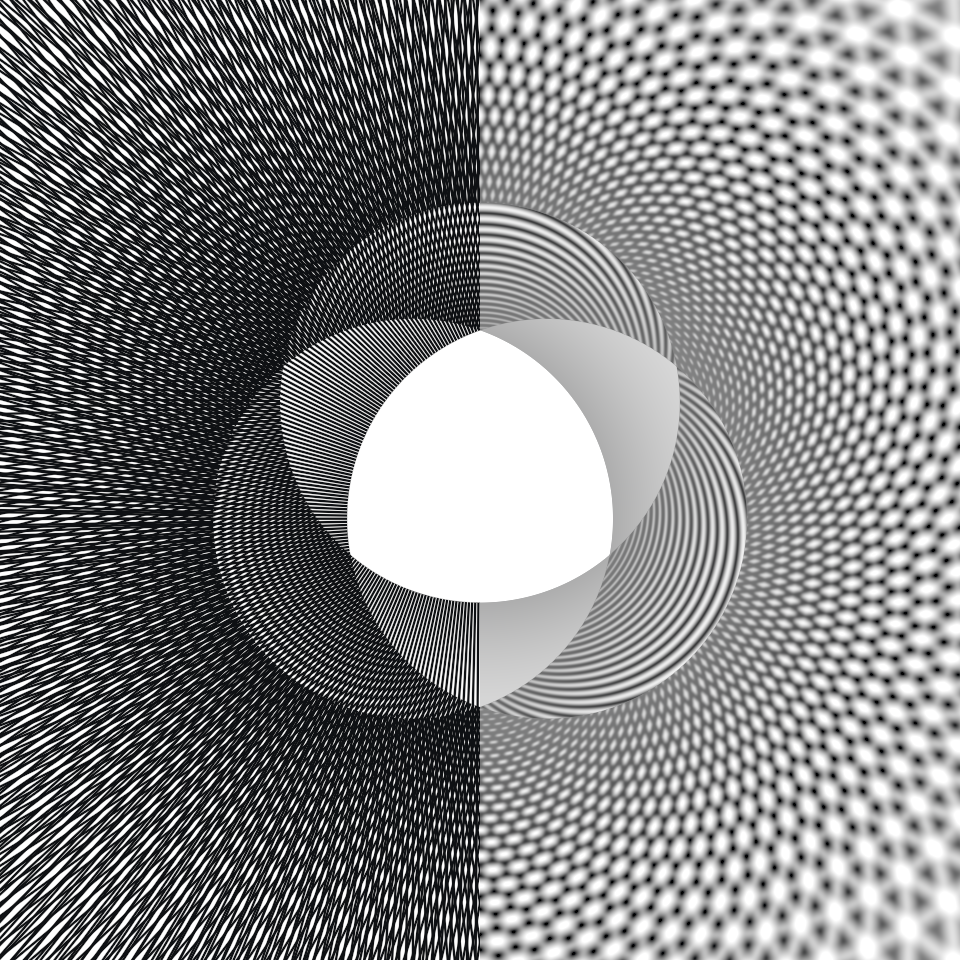
\includegraphics[width=0.62\linewidth]{teaser-fantrio.png}
  \caption{\figlead{Three families, and what pooling sees of them.} Three
  fans of rays from three centres, drawn on the left half and pooled on the
  right. The diagonal slide keeps every recipe whose entries sum to zero,
  so the pooled half is a pattern in all three pairwise differences at
  once, and in their combinations: a rosette that no pair of the fans
  makes alone. Rendered by \Moire\ through its own pooled view
  (\S\ref{sec:instrument}).}
  \label{fig:trio}
\end{figure}

\subsection{What ``emergence'' means here}
\label{sec:emergence}

The word is used loosely often enough that it is worth saying exactly what
is claimed. The third pattern is a new family: it has members and a count,
and the count is a combined count of the parts. It is absent from every
linear description of the parts: an additive superposition has no cross
recipe, so no linear functional of the parts, no spectrum, no filter,
contains it. It appears only to observers that pool after a nonlinearity,
or in superpositions that multiply. And yet its geometry --- where its
members are, how fast its count runs, whether it exists at all --- is fixed
by the parts alone, through $\Phi$, and is the same for every observer that
can see it. That is emergence with a theorem attached, and the theorem is
the last one of this section. It is more abstract than the rest of the
paper; the reader who takes it on trust loses nothing that follows.

\begin{proposition}[The third pattern is the universal invariant]
\label{prop:invariant}
Fix a set of fast directions on the torus, and let $H$ be the set of all
slides along them, by any amount, whole or fractional: the
\emph{rephasings} of the carriers. Let $\E_HI$ be the picture averaged over
all of them. Call a rule $F$ that assigns a number to a picture
\emph{linear} if it respects sums and scalings (an integral of the picture
against any fixed weight is an example). Then every linear rule that gives
the same number for a picture and for every rephased copy of it,
$F(I(\cdot+h))=F(I)$ for all $h$ in $H$, is a function of the averaged
picture alone: $F(I)=F(\E_HI)$. And every rule applied to $\E_HI$ is
unchanged by rephasing. What can be measured of a superposition without
knowing the fast phases is exactly what can be measured of its third
pattern.
\end{proposition}

\begin{proof}
Average the invariance over $H$: $F(I)$ equals the average over $h$ of
$F(I(\cdot+h))$, and a linear rule passes through an average, so that
equals $F$ of the average of $I(\cdot+h)$, which is $F(\E_HI)$. The
converse is that $\E_HI$ is itself unchanged by any further rephasing along
$H$.
\end{proof}

The proposition says that ``the observable content of a superposition, to
anyone who cannot resolve the fast phases, is its tower of averages'' is
not a metaphor. It is the quotient of the picture by the fast rephasing,
in the sense in which a quotient is the most general thing invariant under
a symmetry: whatever two pictures differing only by a rephasing have in
common is a function of their common average, and nothing more. The word
\emph{linear} cannot be dropped --- the picture's energy $\int I^2$ is
unchanged by rephasing and is not a function of the average --- but the
observers that matter physically are not linear rules on the picture; they
are front ends followed by pooling, and for those
Theorem~\ref{thm:universality} already said that the picture is theirs and
the geometry is not. In the philosophers' terms this is \emph{weak}
emergence~\cite{Bedau1997Weak, Chalmers2006Emergence} --- the new pattern
is in principle derivable from the parts --- made exact: a new family, with
a new count, that no member of the parts' description contains, produced
by a quotient that is exact rather than approximate, and exactly computable
at every stage of the hierarchy. It is a better claim than strong
emergence made vague.

\begin{tryit}{a beat of beats}
Three oscillators on a synthesizer, sine waves, at $300$, $330$ and $363$
hertz. You will hear two fast throbs, at thirty and thirty-three per
second, and the question is whether you also hear a slow one, three times a
second. Theorem~\ref{thm:cascade} says a single mild nonlinearity cannot
produce it. Run the mix through a distortion effect and then a low-pass,
one stage: no three-hertz throb should appear. Run it through distortion,
a low-pass at about fifty hertz, and a second distortion: it should. If
your unaided ear hears the slow throb, that is data about the order of your
ear's front end.
\end{tryit}

% Sections not yet written: headings only, so the map in section 1 resolves.
\section{Who can see a beat}
\label{sec:whosees}
\todo{P3: additive versus multiplicative superposition; a nonlinearity mints
a recipe the picture never carried; hard patterns are observer-proof; the
ear model figure.}

\section{Which pattern emerges}
\label{sec:selection}
\todo{P3: selection as slowest per unit of cost; duty nulls; the
continued-fraction ladder; deserts.}

\section{Emergence, iterated}
\label{sec:iterated}
\todo{P3: the emergent pattern is a family; beats of beats need two stages;
the tower property.}

\section{When counting fails}
\label{sec:counting}
\todo{P4: the trichotomy; defects; folds; the Mach number.}

\section{Predictions, measured}
\label{sec:ledger}
\todo{P4: the generated table with a domain column; what is classical, what
is ours, how sure.}

\section{The instrument}
\label{sec:instrument}
\todo{P4: one page on \Moire.}


\bibliographystyle{plain}
\bibliography{refs}

\end{document}
